\section{Flujometrías y CFD}
%
Se realizó una serie de flujometrías para obtener valores de $C_{D}$ en función
de la diferencia de presión a través del puerto y la apertura del
mismo\footnote{ICESym utiliza alzada, por lo que se traduce área de pasaje de
puerto en alzada de válvula equivalente.}, con el fin de obtener un mapa del
coeficiente de descarga en función de la presión y apertura del puerto
($C_{D} = f(\Delta P,l_v)$).
%
ICESym requiere de información del $C_{D}$ para calcular el área efectiva
de pasaje de flujo de las válvulas (o puertos en el caso del MRCVC).
%
Introduciendo el mapa de $C_{D}$ se tiene un mejor modelado del funcionamiento
del sistema de intercambio de gases porque se conoce la pérdida de carga
localizada para un rango de operación del motor.

\nomenclature[PO]{\(\Delta P\)}{Diferencia de Presión entre puerto y cámara}
\nomenclature[PO]{\(l_v\)}{Alzada de válvula o apertura de puerto}


\subsection{Modelos de Turbulencia}
%
El flujo a través del puerto es de carácter transitorio, turbulento; para
modelar este tipo de flujo se utilizó el modelo de turbulencia de dos ecuaciones
\emph{$\kappa-\epsilon$}\parencite{wilcox}, que consta de una ecuación para la
\emph{energía cinética turbulenta} $\kappa$ y otra para la \emph{tasa de
disipación de la energía cinética turbulenta} $\epsilon$.
%
El modelo está basado en el modelo estándar
$\kappa-\epsilon$~\parencite{launderSpalding} y es uno de los más populares con
\emph{performance} conocida.
%
Las ecuaciones del modelo son:

\begin{equation}\label{eq:k}
  \frac{D}{Dt}(\rho \kappa) = \nabla \cdot (\rho D_{\kappa}\nabla \kappa) + P_{\kappa} - \rho \epsilon
\end{equation}

\nomenclature[PO]{\(\rho\)}{Densidad}
\nomenclature[F]{\(\kappa\)}{Energía cinética turbulenta}
\nomenclature[F]{\(\epsilon\)}{Disipación de energía cinética turbulenta}
\nomenclature[F]{\(D_{\kappa}\)}{Difusividad efectiva para $\kappa$}
\nomenclature[F]{\(P_{\kappa}\)}{Tasa de producción de energía cinética turbulenta}
\nomenclature[F]{\(\epsilon\)}{Tasa de disipación de energía cinética turbulenta}

donde

\begin{itemize}
  \item[-] $\kappa$ es la energía cinética turbulenta en $m^{2}s^{-2}$.
  \item[-] $D_{\kappa}$ es la difusividad efectiva para $\kappa$.
  \item[-] $P_{\kappa}$ es la tasa de producción de energía cinética turbulenta en $m^{2}s^{-3}$.
  \item[-] $\epsilon$ es la tasa de disipación de energía cinética turbulenta en $m^{2}s^{-3}$.
\end{itemize}


\begin{equation}\label{eq:k}
  \frac{D}{Dt}(\rho \epsilon) =
  \nabla \cdot (\rho D_{\epsilon}\nabla \epsilon) +
  \frac{C_{1}\epsilon}{\kappa} \left( P_{\kappa}+C_{3}\frac{2}{3}\kappa\nabla\cdot u \right) -
  C_{2}\rho\frac{\epsilon^{2}}{\kappa}
\end{equation}

donde
\begin{itemize}
  \item[-] $D_{\epsilon}$ es la difusividad efectiva de $\epsilon$.
  \item[-] $C_{1}$ es un coeficiente del modelo.
  \item[-] $C_{2}$ es un coeficiente del modelo.
\end{itemize}

La ecuación para la viscosidad turbulenta $\nu_{t}$ es

\begin{equation}\label{eq:nu_t}
  \nu_{t} = C_{\mu}\frac{\kappa^{2}}{\epsilon}
\end{equation}

\nomenclature[F]{\(\nu_{t}\)}{Viscosidad turbulenta}

donde
\begin{itemize}
        \item[-] $C_{\mu}$ es un coeficiente del modelo.
\end{itemize}

Los coeficientes por defecto del modelo son:

% Clossure Coefficient
\begin{equation}
  C_{\epsilon 1}=1,44
  \quad
  C_{\epsilon 2}=1,92
  \quad
  C_{\mu}=0,09
  \quad
  \sigma_{k}=1
  \quad
  \sigma_{\epsilon}=1,3
\end{equation}

El valor inicial para $\kappa$ se puede estimar con:
\begin{equation}\label{eq:kappa_est}
  \kappa = \frac{3}{2} {\left( |u_{ref}| \cdot I \right)}^{2}
\end{equation}

\nomenclature[F]{\(I\)}{Intensidad de turbulencia}

donde
\begin{itemize}
  \item[-] $I$ es la intensidad de turbulencia en \%.
  \item[-] $u_{ref}$ es una velocidad de referencia en $ms^{-1}$.
\end{itemize}

El valor inicial para $\epsilon$ se puede estimar con:
\begin{equation}\label{eq:epsilon_est}
  \epsilon = \frac{{C_{\mu}}^{3/4} \cdot {\kappa}^{3/2}} {l_{m}}
\end{equation}

donde
\begin{itemize}
 \item[-] $l_{m}$ es una longitud de referencia, para flujos internos se estima
con el diámetro hidráulico de la cañería, usando por ejemplo $0,07 \cdot D_{m}$.
\end{itemize}

\nomenclature[F]{\(l_m\)}{Longitud de mezcla o escala de viscosidad}

% https://www.openfoam.com/documentation/guides/latest/doc/guide-turbulence-ras-k-epsilon.html

Las ecuaciones anteriores de  $\kappa$ y $\epsilon$ son estimaciones para dar un
valor inicial al problema.
%
La longitud de mezcla $l_m$ determina el tamaño que pueden tener los torbellinos
turbulentos, su valor inicial se aproximó como la altura de cámara $l_m = h_c$.
%

\subsection{Condiciones Iniciales}\label{cap2:cond_iniciales}
%
Las condiciones iniciales se determinan para cada diferentes puntos operativos
de interés del motor a partir de los datos obtenidos del simulador ICESym.
%
Se tienen dos casos distintivos al momento de modelar el flujo a través de los
puertos: flujo compresible e incompresible.
%
Para este último se considera que los efectos de la compresibilidad del gas se
pueden despreciar cuando el número de Mach es menor a $0,3-0,4$.
%
Además, se deben separar los casos a modelar entre aquellos en los que hay
solape de cámaras y los que no (ver Figura~\ref{fig:solape}).
%
En estos casos se define también un valor medio para inicializar el interior del
dominio que representa el gas dentro de la cámara de combustión.

\begin{figure}[t!]
  \centering
    \begin{subfigure}[t]{0.4\textwidth}
        \centering
        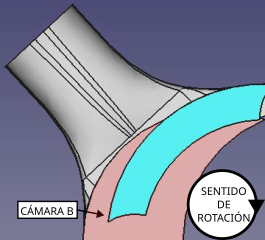
\includegraphics[width=\textwidth]{flujometrias/sin_solape.png}
        \caption{Sin solape}
    \end{subfigure}%
    \begin{subfigure}[t]{0.4\textwidth}
        \centering
        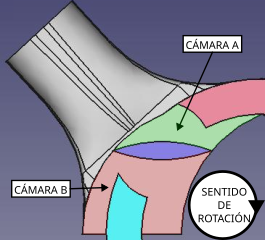
\includegraphics[width=\textwidth]{flujometrias/con_solape.png}
        \caption{Con solape}
    \end{subfigure}
  \caption{Solape de cámaras}\label{fig:solape}
\end{figure}

Independientemente del tipo de flujo que se esté simulando, de ICESym se toman
los valores de presión, temperatura, densidad y velocidad para calcular los
valores iniciales.

Debido a la cantidad de flujometrías a realizar, se utilizó un \emph{script} para leer
los datos de salida de ICESym y calcular los valores requeridos en función del
tipo de flujo a simular.
%
Este \emph{script} toma el estado del gas del simulador tanto en la cámara de
combustión como del puerto que se esté analizando, para la posición de alzada y
RPM requeridas.
%
Con estos valores se calculan las propiedades termodinámicas del gas con las
siguientes relaciones para cada cámara analizada, los valores leídos son:

\begin{itemize}
    \item $\rho_{c,i}$, es la densidad del gas en la cámara $i$.
    \item $P_{c,i}$, es la presión del gas en la cámara $i$.
    \item $T_{c,i}$, es la temperatura del gas en la cámara $i$.
    \item $\rho_{p,i}$, es la densidad del puerto $i$.
    \item $v_{p,i}$, es la velocidad del gas en el puerto $i$.
    \item $P_{p,i}$, es la presión del gas en el puerto $i$.
\end{itemize}

Con estos valores iniciales se pueden calcular o estimar las propiedades
termodinámicas de la mezcla de gases frescos o quemados, dependiendo si se está
evaluando un puerto de admisión o escape, los valores calculados son:
%
\begin{itemize}
    \item $M_{M}$, masa molar, ec.(\ref{eq:mw})
    \item $C_{p}$, calor específico a presión constante
    \item $\gamma$, relación $C_{p}/C_{v}$ del gas
    \item $\mu$, viscosidad dinámica, ec.(\ref{eq:mu})
    \item $\nu$, viscosidad cinemática
    \item $P_{R}$, número de Prandtl, ec.(\ref{eq:pr})
    \item $k_{est}$, energía cinética turbulenta, ec.(\ref{eq:kappa_est})
    \item $\epsilon_{est}$, disipación de la energía cinética turbulenta, ec.(\ref{eq:epsilon_est})
\end{itemize}

\nomenclature[F]{\(M_{M}\)}{Masa molar}
\nomenclature[F]{\(C_{p}\)}{Calor específico a presión constante}
\nomenclature[F]{\(\gamma\)}{Cociente de calores específicos}
\nomenclature[F]{\(\mu\)}{Viscosidad dinámica}
\nomenclature[F]{\(\nu\)}{Viscosidad cinemática}
\nomenclature[F]{\(P_{R}\)}{Número de Prandtl}
\nomenclature[F]{\(k_{est}\)}{Energía cinética turbulenta}
\nomenclature[F]{\(\epsilon_{est}\)}{Disipación de la energía cinética turbulenta}


Para simplificar el análisis no se tuvo en cuenta la fracción de gases
residuales.
%
El gas ``flujado'' es siempre aire limpio en el caso de los puertos
de admisión o el gas quemado de una mezcla estequiométrica de aire-combustible
en caso de los puertos de escape, siendo isooctano $C_{8}H_{18}$ el combustible
seleccionado.
%
Las ecuaciones utilizadas para modelar las propiedades termodinámicas de las
mezclas aire-combustible fueron descritas brevemente en la
sección~\ref{subsec:prop_mezcla}.

\subsection{Malla}

La malla se construyó a partir del modelo de CAD generado con los resultados
obtenidos de las simulaciones del motor.
%
La implementación de las diferentes herramientas requeridas para generar una
malla apta para realizar las flujometrías se describe en el
apartado~\ref{sec:cap3_of_malla}.

El grado de refinamiento de la misma se determinó luego de realizar una serie de
flujometrías con tamaños decrecientes de celda y viendo la variabilidad de los
resultados.
%
El objetivo de las flujometrías es obtener el flujo másico $\dot{m}$ del puerto
para un estado del gas dado.
%
Se redujo el tamaño inicial de celda hasta que el valor de $\dot{m}$ no se
modificó en más de un 5\% del valor anterior, con un nivel de refinamiento
mayor.
%
En algunos casos se utilizaron los resultados de flujometrías con mallas menos
refinadas como valor inicial de una malla de mayor refinamiento con el propósito
de reducir el tiempo total de simulación.
%
Por ejemplo, con una malla inicial de cubos de 15mm de lado se obtiene una
solución que se usa como valor inicial para una malla de 10mm, a su vez este
resultado se utiliza como valor inicial de la simulación final con una malla de
cubos de 5mm de lado para obtener el valor de $\dot{m}$ utilizado para calcular
el $C_{D}$.

Este proceso se representa para el caso del puerto de admisión a $0^{\circ}$ y
$120^{\circ}$ con el motor girando a 2000 RPM.
%
Se simuló el puerto con tamaños de malla iniciales de 20, 10, 5 y 2,5 mm,
evaluando la variación del caudal con la cantidad de celdas de la malla, ver
Figuras~\ref{fig:refinamiento} y~\ref{fig:conv_malla}.

\begin{figure}[ht]
  \centering
  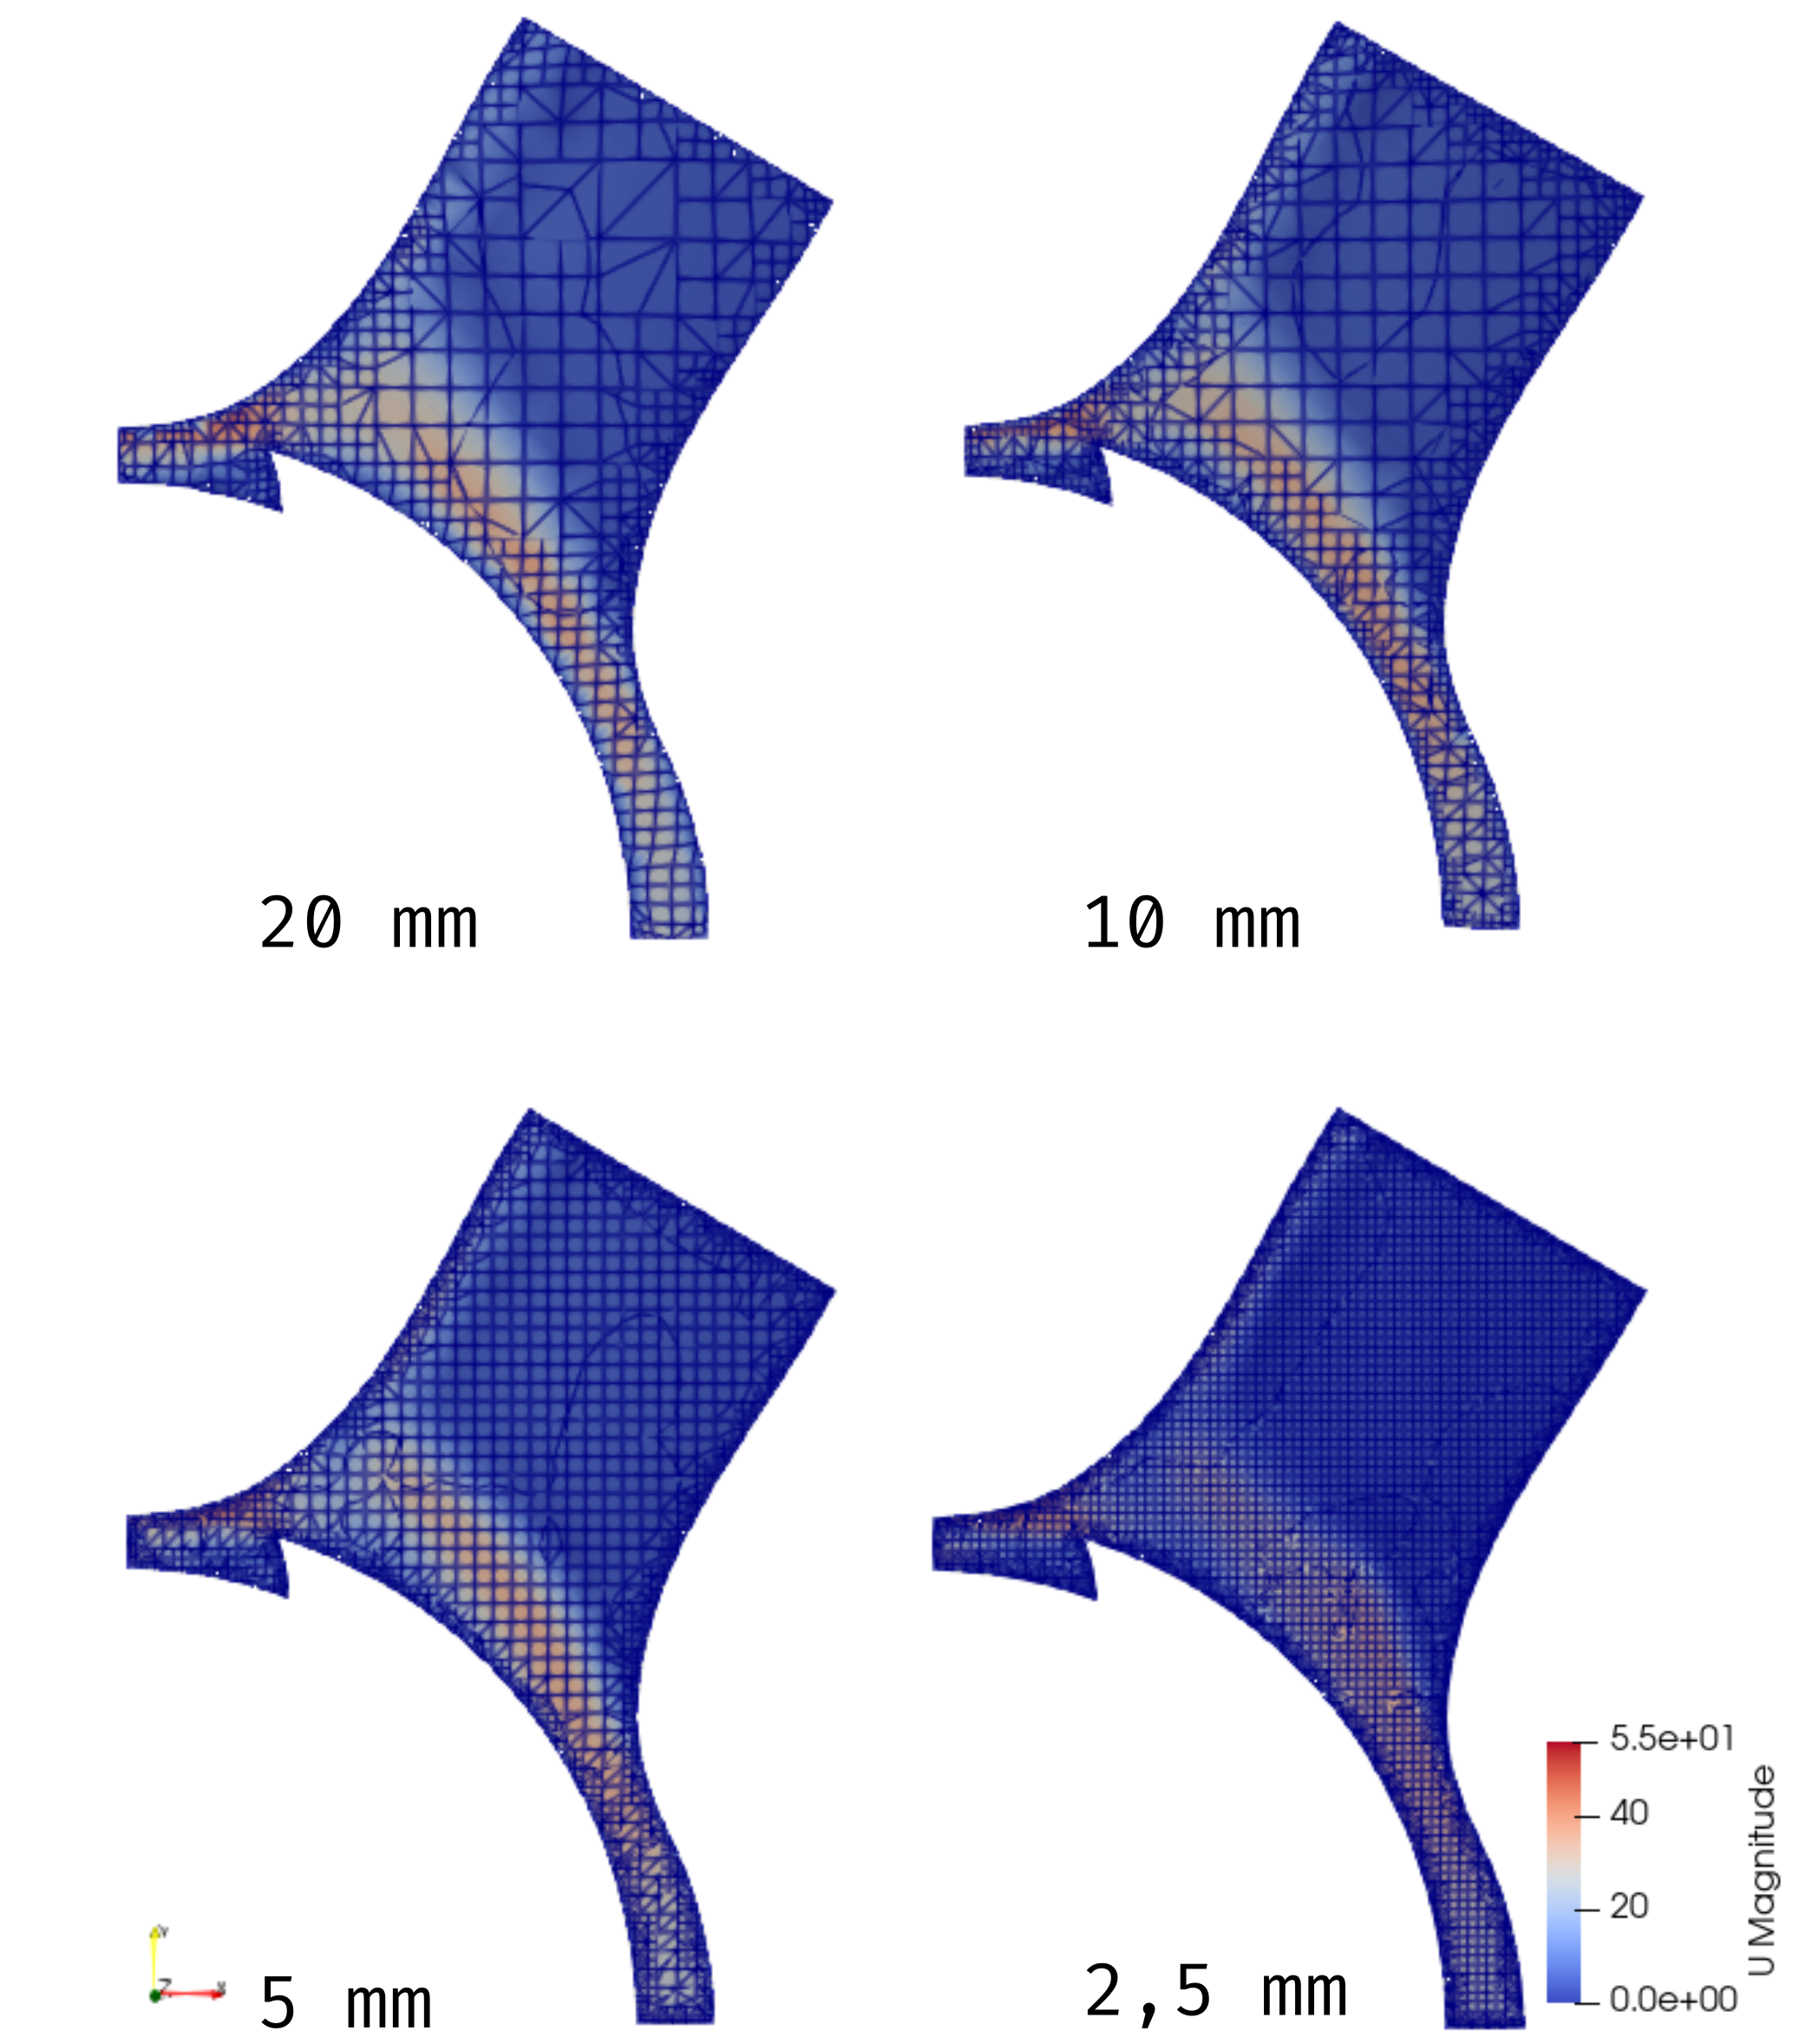
\includegraphics[width=0.8\textwidth]{./flujometrias/refinamiento_malla.png}
  \caption{Refinamiento de malla}\label{fig:refinamiento}
\end{figure}

\begin{figure}[ht]
  \centering
  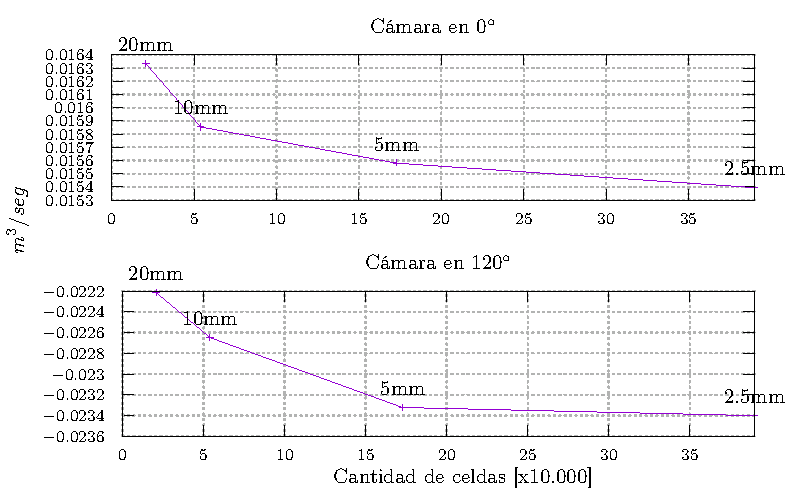
\includegraphics[width=0.9\textwidth]{./flujometrias/convergencia_admision_2000rpm.pdf}
  \caption{Convergencia de malla de puerto de admisión}\label{fig:conv_malla}
\end{figure}


\subsection{Coeficiente de Descarga $C_{D}$}\label{sec:cap2_cd}

La pérdida de carga localizada en los puertos de admisión y escape se puede
representar a través del coeficiente de descarga, $C_{D}$.
%
El valor de $C_{D}$ varía con la geometría y condiciones de operación del
puerto, siendo $C_{D}=1$ el caso ideal sin pérdida de carga localizada.
%
El $C_{D}$ es un parámetro importante porque permite obtener una mejor estimación
del flujo másico real en el puerto, se define como:

\begin{equation}
  C_{D} = \frac{\text{flujo másico real}}{\text{flujo másico ideal}}
\end{equation}

El valor de $C_{D}$ de un puerto se puede obtener experimentalmente con un
flujómetro, el ensayo consiste en medir el caudal que circula por un puerto con
una presión de descarga fija que, dependiendo del fabricante del equpo varía
entre 250-700 mm.c.a.
%
Comúnmente estos ensayos se realizan en un banco que incluye solamente la tapa
de cilindros, dejando de lado otros elementos del sistema como el pistón y los
conductos de admisión.
%
Durante el ensayo se mide el caudal de aire atmosférico para diferentes grados
de apertura de la válvula y así se obtienen datos de (alzada, flujo) con los
cuales comparar entre diferentes geometrías del puertos de admisión o escape.
%
En la imagen~\ref{fig:banco_flujometrias} se muestra un banco de pruebas
comercial.


\begin{figure} \centering
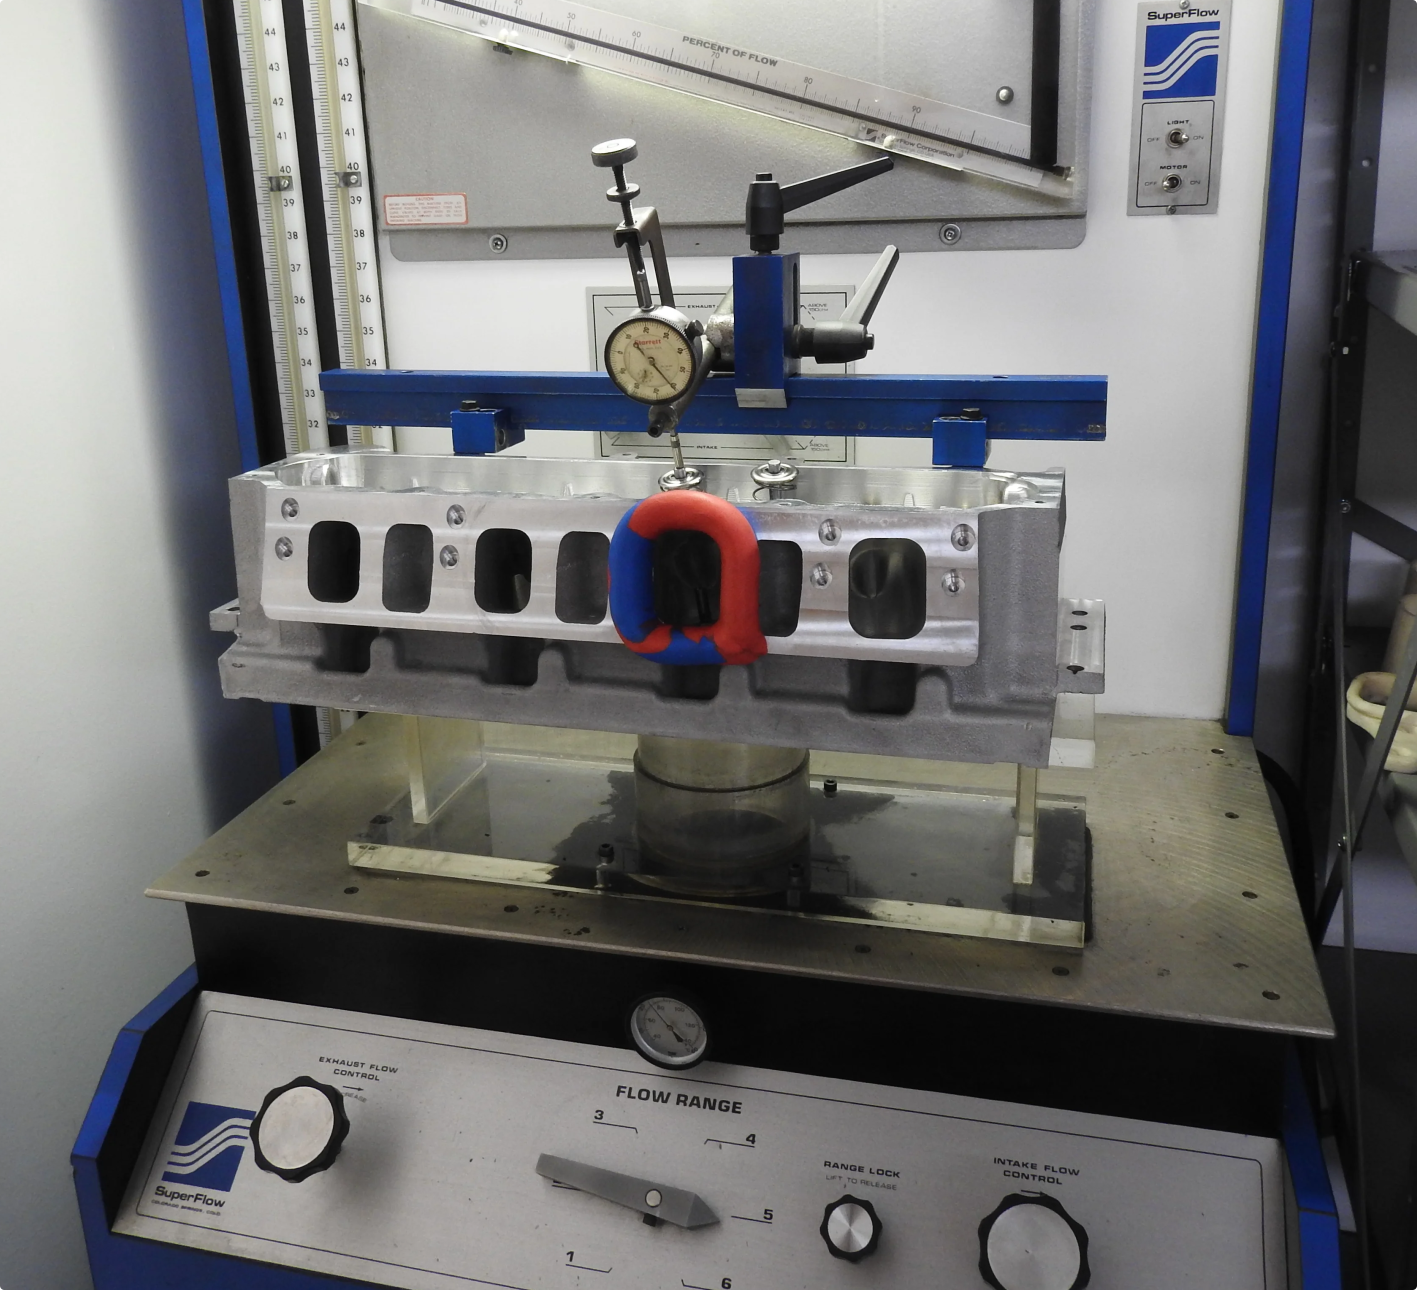
\includegraphics[width=0.7\textwidth]{./flujometrias/banco_flujometrias.png}
  \caption{Banco de flujometrías Super-Flow SF-750}\label{fig:banco_flujometrias}
\end{figure}

Otra forma de obtener un coeficiente de descarga es por medio de flujometrías
computacionales, el uso de CFD permite modelar el puerto en condiciones
operativas, incluyendo la interacción con elementos como por ejemplo el pistón,
o en el caso del MRCVC, estator y conjunto rotante.
%
Además, se puede modelar las propiedades del fluido de trabajo para una
viscosidad, presión y temperatura representativas de las condiciones operativas
del motor.

El valor de $C_{D}$ se obtiene de las ecuaciones de flujo másico $\dot{m}$ que
circula a través del puerto, el cual se calcula a partir de las ecuaciones de
flujo compresible a través de una restricción, habiendo dos casos distintivos:
flujo bloqueado y no bloqueado.

Para el caso en que el flujo no esté bloqueado la ecuación de $\dot{m}$ es
la~(\ref{eq:m_no_bloqueado}) y en caso de que se cumpla la
desigualdad~(\ref{eq:cond_bloqueo}) el flujo está bloqueado y se utiliza la
ecuación~(\ref{eq:m_bloqueado}):
%

\begin{equation}\label{eq:m_no_bloqueado}
  \dot{m} = \frac{C_D A_R p_0}{\sqrt{R T_0}} {\left(\frac{p_T}{p_0} \right)}^{1/\gamma} {\left( \frac{2\gamma}{\gamma-1} \left[1- {(\frac{p_T}{p_0})}^{{\gamma-1}/\gamma} \right] \right)}^{1/2}
\end{equation}

\begin{equation}\label{eq:cond_bloqueo}
  \frac{p_T}{p_0} \le {[\frac{2}{\gamma+1}]}^{\gamma/(\gamma - 1)}
\end{equation}

\begin{equation}\label{eq:m_bloqueado}
  \dot{m}=  \frac {C_D A_R p_0} {{(R T_0)}^{1/2}} \gamma^{1/2} {\left( \frac{2\gamma}{\gamma+1} \right)}^{(\gamma+1)/(2(\gamma-1))}
\end{equation}

donde
\begin{itemize}
    \item $p_0$, es la presión de estancamiento antes de la restricción.
    \item $T_0$, es la temperatura de estancamiento antes de la restricción.
    \item $p_T$, es la presión estática justo después de la restricción.
    \item $A_R$, es el área de pasaje de flujo o de referencia.
    \item $\dot{m}$, es el caudal másico.
  \item $\gamma$, es el cociente de capacidades térmicas del gas.
\end{itemize}

\nomenclature[PO]{\(p_0\)}{Presión de estancamiento antes de la restricción}
\nomenclature[PO]{\(T_0\)}{Temperatura de estancamiento antes de la restricción}
\nomenclature[PO]{\(p_T\)}{Presión estática justo después de la restricción}
\nomenclature[G]{\(A_R\)}{Área de pasaje de flujo o de referencia}

El flujo está bloqueado si la velocidad en la garganta de la restricción alcanza
la velocidad sónica, dada esta condición $\dot{m}$ alcanza un límite y reducir
la presión aguas abajo de la restricción no produce un aumento del caudal.
%
% La condición de flujo bloqueado se puede expresar en términos de la relación de
% presiones aguas arriba $p_{0}$ y aguas abajo de la restricción $p_{T}$.
%
Las presiones y temperaturas involucradas en el cálculo de $\dot{m}$ se pueden
medir u obtener de una simulación computacional del ciclo del motor.
%
\nomenclature[PO]{\(p,P\)}{Presión}

Un parámetro importante en las ecuaciones utilizadas para el cálculo del
coeficiente de descarga $C_{D}$ es el área de referencia $A_{R}$ que define el
área utilizada para calcular el caudal másico que circula por el puerto.
%
% En un motor con válvulas se suele tomar el área de cortina como el producto de
% la circunferencia de la válvula con la alzada, es decir:

La elección del área de referencia utilizada para el cálculo es arbitraria, sin
embargo en un motor con válvulas se suele utilizar el área de cortina
(ver~\ref{fig:area_cortina}), que se calcula con el producto del diámetro
$D_{v}$ y alzada de válvula $l_{v}$:

\begin{equation} \label{eq:area_cortina}
  A_R = A_C = \pi D_v l_v
\end{equation}

\begin{equation}\label{eq:ar_cortina}
  A_{R}=\pi D_{v} \cdot h_{v}
\end{equation}

\nomenclature[G]{\(A_R\)}{Área de pasaje de flujo o de referencia}
\nomenclature[G]{\(h_v\)}{Alzada de válvula}
\nomenclature[G]{\(A_C\)}{Área de cortina}
\nomenclature[G]{\(D_v\)}{Diámetro de válvula}
\nomenclature[G]{\(l_v\)}{Alzada de válvula}

\begin{figure} \centering
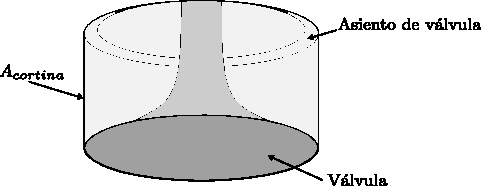
\includegraphics[width=0.5\textwidth]{valve_curtain.pdf}
  \caption{Área de cortina}\label{fig:area_cortina}
\end{figure}

El área de referencia utilizada en ICESym es el área frontal del puerto expuesta
a la cámara que se esté analizando, calculada como:

\begin{equation}\label{eq:ar_mrcvc}
  A_{R} = h_{p} \cdot l_{v}
\end{equation}

El área de cortina se ilustra en la Figura~\ref{fig:area_cortina} y el área
utilizada en ICESym para el MRCVC en la Figura~\ref{fig:area_referencia}.
%
En esta última figura se observan dos zonas coloreadas, que hacen referencia al
área de dos cámaras durante el solape que ocurre por la geometría del motor.

\begin{figure}
  \centering
  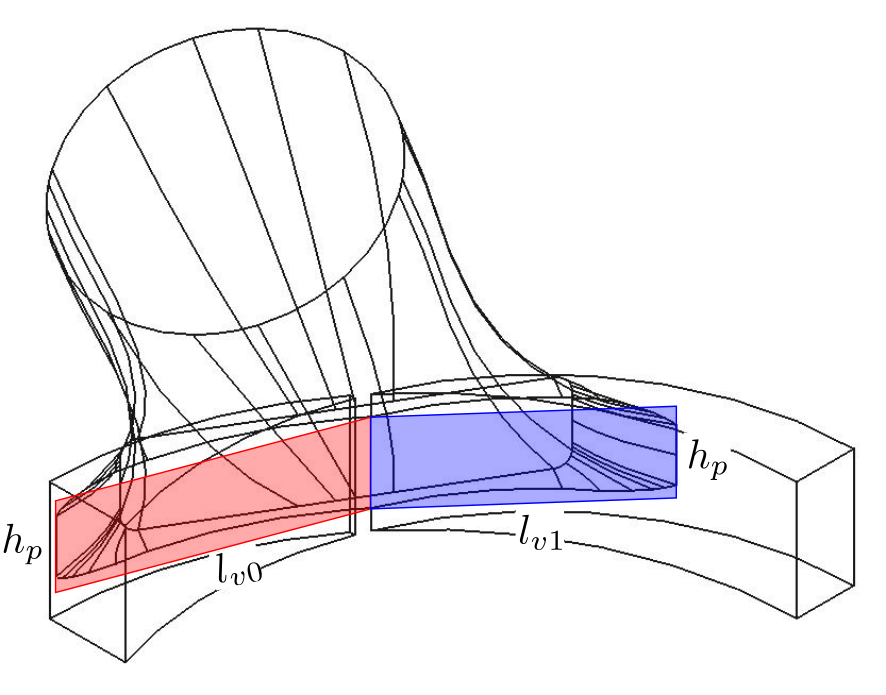
\includegraphics[width=.7\textwidth]{area_referencia.png}
  \caption{Área de referencia MRCVC}\label{fig:area_referencia}
\end{figure}

Los valores de densidad, velocidad, presión y temperatura se obtienen de los
datos de salida de ICESym para un puerto, ángulo y velocidad dada.
%
Para la temperatura se utiliza la temperatura de la cámara, $T_0 = T_C$, la
presión antes y después del puerto se selecciona de acuerdo al sentido de flujo,
en caso de ser hacia la cámara de combustión la presión en el puerto se utiliza
como inicial $P_0$ y la presión en la cámara es la aproximación a la presión en
la restricción $P_T$.
\nomenclature[PO]{\(T\)}{Temperatura}
\nomenclature[SU]{\(0\)}{Valor inicial}

El valor de $\gamma$ se obtiene de las propiedades de la mezcla con las rutinas
computacionales descritas en el apartado~\ref{subsec:prop_mezcla}.

De las flujometrías se obtiene el caudal másico que fluja el puerto, con este
dato y las ecuaciones anteriores se puede determinar el valor de $C_{D}$.

\subsection{Esquemas de Discretización}

Se utilizan para resolver ecuaciones de variables continuas con funciones
discretas en tiempo y espacio.
%
Se deben seleccionar esquemas para resolver:

\begin{itemize}
  \item Primera derivada temporal
  \item Interpolación
  \item Gradiente
  \item Divergencia
  \item Gradientes normales a superficies
  \item Laplacianos
\end{itemize}


\paragraph{Derivadas temporales, $\delta / \delta t$}
%
Estas derivadas se discretizan con el método de Euler\parencite{burden}, que
aproxima la integración de un paso $n$ a $n+1$ con $y_{n+1}-y_{n}\simeq hf_{n}$
donde $h = t_{n+1}-t_{n}$ es el paso temporal y $f_{n}=f(t_{n},y_{n})$.
%
Para el esquema de Euler hacia atrás la aproximación es
$y_{n+1}-y_{n}\simeq h f_{n+1}$.
%
A este esquema se le agrega un coeficiente $\gamma\in[0,1]$ de modo que:

\begin{equation}
  y_{n+1}-y_{n} \simeq \gamma h f_{n+q} + (1-\gamma)h f_{n}
\end{equation}

Con $\gamma=1/2$ el esquema es equivalente a Crank-Nicolson estándar, se puede
convertir al esquema de Euler hacia adelante con $\gamma=0$.

\paragraph{Gradientes}
%
Se discretiza utilizando integración Gaussiana con interpolación lineal entre
valores de celdas.
%
El método define al gradiente medio en un elemento de volumen finito con
centroide \textbf{C} y volumen $V_{c}$ en términos de los flujos a través de sus
caras, como lo indica la ecuación~(\ref{eq:green_gauss_gradient}).
%
Para esto se requiere conocer los valores de la variable $\phi_{f}$ en las caras
vecinas e información del área de la celda y su normal $(\vec{S}_{f})$.

\begin{equation}
  \label{eq:green_gauss_gradient}
  \nabla \phi_{P} = \frac{1}{V_{c}}\sum_{f} \vec{S}_{f}\phi_{f}
\end{equation}

El método de volúmenes finitos utiliza valores en las caras de las celdas, por
lo que se debe aproximar el valor de la variable en una cara dada para obtener
el valor del gradiente en dicha celda.
%
Los valores de $\phi_{f}$ se obtienen de una interpolación lineal entre valores
conocidos de celdas adyacentes.
%
Un método de interpolación entre celdas puede ser:

\begin{align}
  \label{eq:interpolacion_lineal_caras}
  \alpha &= \frac{|{\vec{r}_{N}-\vec{r}_{f}}|} {|{\vec{r}_{N}-\vec{r}_{P}}|}\\
  \phi_{f} &= \alpha\phi_{P}+(1-\alpha)\phi_{N} \\
\end{align}

Donde $\alpha$ es un factor de ponderación geométrico entre las celdas \textbf{P} y
\textbf{N} y $\vec{r}$ es un vector de posición.

La interpolación se puede limitar para que los valores obtenidos se encuentren
entre el mínimo y máximo de las celdas vecinas, este método se denomina
``limitado''.


%Gradiente normal a la superficie
\paragraph{Gradiente normal a una superficie}
%
Este gradiente es evaluado en la cara de la celda.
%
Es la componente (normal a la cara) del gradiente entre los valores de los
centroides de 2 celdas conectadas por la cara evaluada.
%
En general las mallas utilizadas para modelar geometrías reales no son
ortogonales.
%
Esto hace que un vector $S_{f}$ normal a una superficie no necesariamente sea
colineal con el vector que une el centroide de dos celdas contiguas.
%
El gradiente en la cara en la dirección que une los centroides (C y F) de las
celdas $\vec{e}$ es

\begin{equation}
  \label{eq:gradiente_normal}
  (\nabla \phi \cdot \vec{e_{f}}) = \frac{\nabla\phi}{\delta n} = \frac{\phi_{F} - \phi_{C}}{||\vec{r_{C}}-\vec{r_{F}}||} = \frac{\phi_{F} - \phi_{C}}{d_{CF}}
\end{equation}

Donde el subíndice \textbf{f} indica que se evalúa en la cara de una celda.
%
El vector de superficie $S_{f}$ se puede escribir en términos de sus componentes
normal y tangente a la cara $f$ en la que es evaluado.

\begin{equation}
  \vec{S_{f}}= \vec{E_{f}} + \vec{T_{f}}
\end{equation}

De esta forma, el gradiente del flujo de la variable $\phi$ en mallas no
ortogonales se puede expresar en términos de las componentes normal y tangente a
la cara de la celda~\parencite{moukalled}.
%
El término \textbf{E} indica el flujo de $\phi$ normal a la cara y \textbf{T} el
flujo tangente.

\begin{align}
  \label{eq:gradiente}
  %
  {(\nabla \phi)}_{f}\cdot \vec{S_{f}} &= {(\nabla \phi)}_{f}\cdot E_{f} + {(\nabla \phi)}_{f}\cdot \vec{T_{f}} \\
  %
  &= \vec{E_{f}}\frac{\phi_{F}-\phi_{C}}{d_{FC}}+ {(\nabla \phi)}_{f}\cdot \vec{T_{f}}
\end{align}

%
Algunos esquemas de discretización de este tipo de gradientes son:
\begin{itemize}
  \item No corregido
  \item Ortogonal
  \item Corregido y limitado
\end{itemize}

La corrección ortogonal rota el vector $S_{f}$ hasta que sea normal a la superficie.
%
La corrección limitada aplica la corrección ortogonal, sumando
$\cos^{-1}{\theta}$, donde $\theta$ es el ángulo entre la normal a la cara y el
vector $S_{f}$.

% Divergencia
\paragraph{Divergencia}
%
Se utiliza un esquema de integración Gaussiana con interpolación lineal para
la discretización de la divergencia.

Dependiendo de los tipos de variable, se utilizan diferentes esquemas de
interpolación disponibles son:
%
\begin{itemize}
        \item centrada
        \item hacia adelante
        \item hacia atrás
        \item limitada
\end{itemize}

\paragraph{Laplacianos}
%
Los términos Laplacianos se discretizan utilizando integración Gaussiana con
interpolación lineal.


\subsubsection{Resumen de Esquemas Seleccionados}
%
Los esquemas de discretización utilizados fueron, para el caso de \textbf{flujo
incompresible}:

\begin{itemize}
  \item Tiempo: Euler hacia atrás
  \item Gradiente:
        \begin{itemize}
                \item $\nabla p$: Integración Gaussiana con interpolación lineal
                \item $\nabla U$: Integración Gaussiana con interpolación lineal
        \end{itemize}
  \item Divergencia:
        \begin{itemize}
                \item $\nabla\cdot (\phi U)$: Integración Gaussiana con interpolación lineal de segundo orden, hacia adelante limitada con $\nabla U$
                \item $\nabla\cdot (\phi k)$: Integración Gaussiana con interpolación lineal hacia adelante
                \item $\nabla\cdot (\phi \epsilon)$: Integración Gaussiana hacia adelante con interpolación lineal
                \item $\nabla\cdot (\phi R)$: Integración Gaussiana con interpolación lineal
                \item $\nabla\cdot R$: Integración Gaussiana con interpolación lineal
                \item $\nabla\cdot \nu_{eff}$: Integración Gaussiana con interpolación lineal

        \end{itemize}
  \item Laplacianos: Integración Gaussiana con interpolación lineal
  \item Interpolación: Lineal
  \item Gradientes normales a la superficie: sin corregir
\end{itemize}

Donde $\phi$ es el flujo volumétrico en la cara de la celda.
%
Para los casos de \textbf{flujo compresible}:

\begin{itemize}
        \item Esquemas temporales: Euler
        \item Gradientes: Integración Gaussiana con interpolación lineal limitada por las celdas.
        \item Divergencia:
        \begin{itemize}
                \item $\nabla \cdot (\phi U)$: Integración Gaussiana con interpolación lineal de segundo orden, hacia adelante limitada con $\nabla U$
                \item $\nabla \cdot (\phi,e)$: Integración Gaussiana con interpolación lineal limitada
                \item $\nabla \cdot (\phi,h)$: Integración Gaussiana con interpolación linear hacia adelante
                \item $\nabla \cdot (\phi,p)$: Integración Gaussiana con interpolación lineal limitada
                \item $\nabla \cdot (\phi,K)$: Integración Gaussiana con interpolación lineal
                \item $\nabla \cdot (\phi,p)$: Integración Gaussiana con interpolación lineal limitada
                \item $\nabla \cdot (\phi,k)$: Integración Gaussiana con interpolación lineal
                \item $\nabla \cdot (\phi,\epsilon)$: Integración Gaussiana con interpolación lineanl hacia adelante
                \item $\nabla \cdot (((\rho\cdot \nu_{Eff}) dev2((\nabla U)^{T})))$ Integración Gaussiana con interpolación lineal
        \end{itemize}
        \item Laplacianos: Integración Gaussiana con interpolación lineal, limitada y corregida
        \item Interpolación: lineal
        \item Gradientes normales a la superficie: corregida
\end{itemize}

Donde $\phi$ es el flujo másico en la cara de la celda.

% Otros
%
% Para inicializar el campo de presión y densidades, se usa la media entre las
% cámaras que se estén simulando y se establece un campo uniforme.

% La velocidad se inicializa con un campo nulo de velocidades, que en la
% configuración de OpenFOAM se designa como \emph{internalField uniform (0 0 0)}.

% En resumen, los valores iniciales de los campos de presión, temperatura y velocidad
% son los indicados en la tabla~\ref{tab:cc}.

% % \begin{table}
% % \centering
% %     \begin{tabular}{cccc} \toprule
% %         Var & Campo         & Parche                      & Pared \\
% %         T   & uniforme T0   & inletOutlet                 & uniforme T9\\ \midrule
% %         P   & uniform Pavg  & uniformTotalPressure        & Pi \\
% %         U   & uniform (0 0 0) & pressureInletOutletVelocity & valor fijo (0 0 0)\\
% %         rho & uniform rhoAvg \\ \bottomrule
% %     \end{tabular}
% %     \caption{Condiciones de Borde}\label{tab:cc}
% % \end{table}

% En todos los casos se tomará como velocidad de referencia a la media entre la
% velocidad en la punta del tubo de las cámaras solapadas.
% %
% Del mismo modo, la temperatura será la temperatura de cámara media.

% Si hay o no solape de cámaras va a depender tanto de la geometría del puerto
% como de la posición del ciclo en la que se encuentre, para determinar las
% condiciones iniciales se debe tener en cuenta el solape.
% %
% En la Figura~\ref{fig:geom} se muestra un corte del puerto con un plano cuya
% normal está en $\vec{z}$, se denominará a la cámara que esté a la izquierda
% como cámara 0 y a la que esté a la derecha cámara 1.
% %
% Al haber solape de cámaras, para definir la presión del puerto y estimar las
% condiciones iniciales de los parámetros viscosos que requiere el modelo
% $k-\epsilon$ se utilizan valores medios de presión, velocidad y temperatura de
% ambas cámaras.
% %
% Además, las condiciones iniciales que se aplican al parche denominado
% \emph{puerto} es igual a la media aritmética de la velocidad de las velocidades
% de los puertos de ambas cámaras, Lo mismo sucede con la presión, densidad y
% temperatura.

% A partir de estos datos se calculan varias propiedades termodinámicas del gas,
% incluyendo la constante del gas, masa molar, viscosidad cinemática y demás.
% %
% Para calcular estas propiedades se asume que el gas no contiene gases
% residuales.

% Finalmente el caudal másico yse obtiene con OpenFOAM, en donde se simula el
% tiempo suficiente para que los caudales másicos por entradas o salidas se
% estabilice, como se ve en la Figura~\ref{fig:caudalMasico}.

% \begin{figure}
%     \centering
%     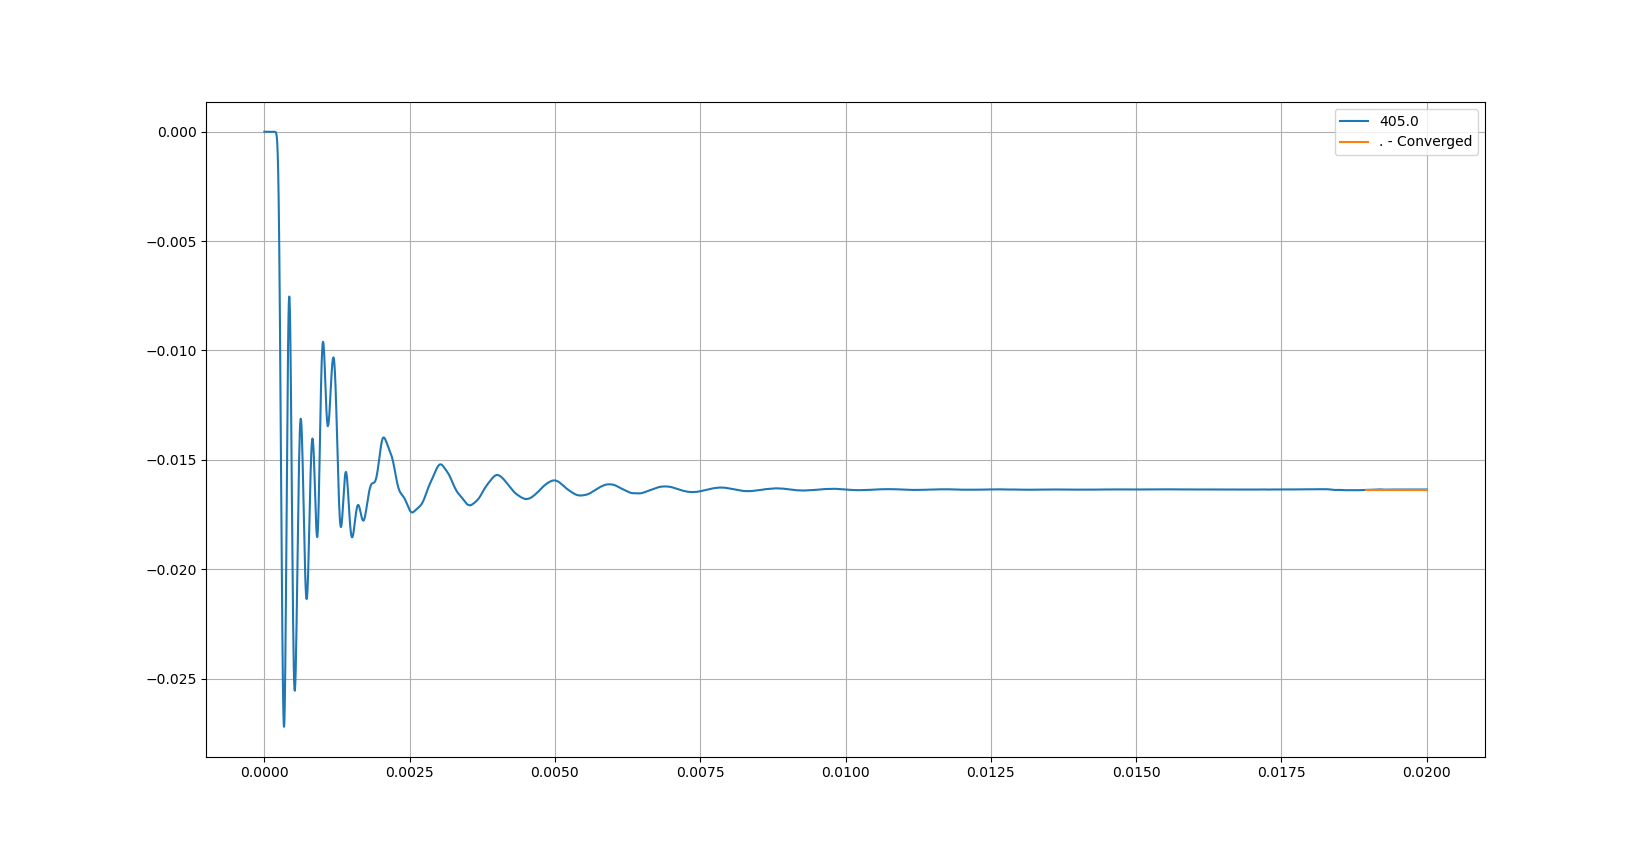
\includegraphics[width=0.6\textwidth]{surfaceFieldValue_405.0.png}
%     \caption{Flujometrías para el puerto de Admisión}\label{fig:caudalMasico}
% \end{figure}

% En todos los casos se tomará como velocidad de referencia a la media entre la
% velocidad en la punta del tubo de las cámaras que se estén solapando.
% %
% Del mismo modo, la temperatura será la temperatura de cámara media.

% Si hay o no solape de cámaras va a depender tanto de la geometría del puerto
% como de la posición del ciclo en la que se encuentre, para determinar las
% condiciones iniciales se debe tener en cuenta el solape.
% %
% En la Figura~\ref{fig:geom} se muestra un corte del puerto con un plano cuya
% normal está en $\vec{z}$, se denominará a la cámara que esté a la izquierda
% como cámara 0 y a la que esté a la derecha cámara 1
% %
% Al haber solape de cámaras, para definir la presión del puerto y estimar las
% condiciones iniciales de los parámetros viscosos que requiere el modelo
% $k-\epsilon$ se utilizan valores medios de presión, velocidad y temperatura de
% ambas cámaras.
% %
% Además, las condiciones iniciales de que se aplican al parche denominado
% \emph{puerto} es igual a la media aritmética de la velocidad de las velocidades
% de los puertos de ambas cámaras, Lo mismo sucede con la presión, densidad y
% temperatura.
